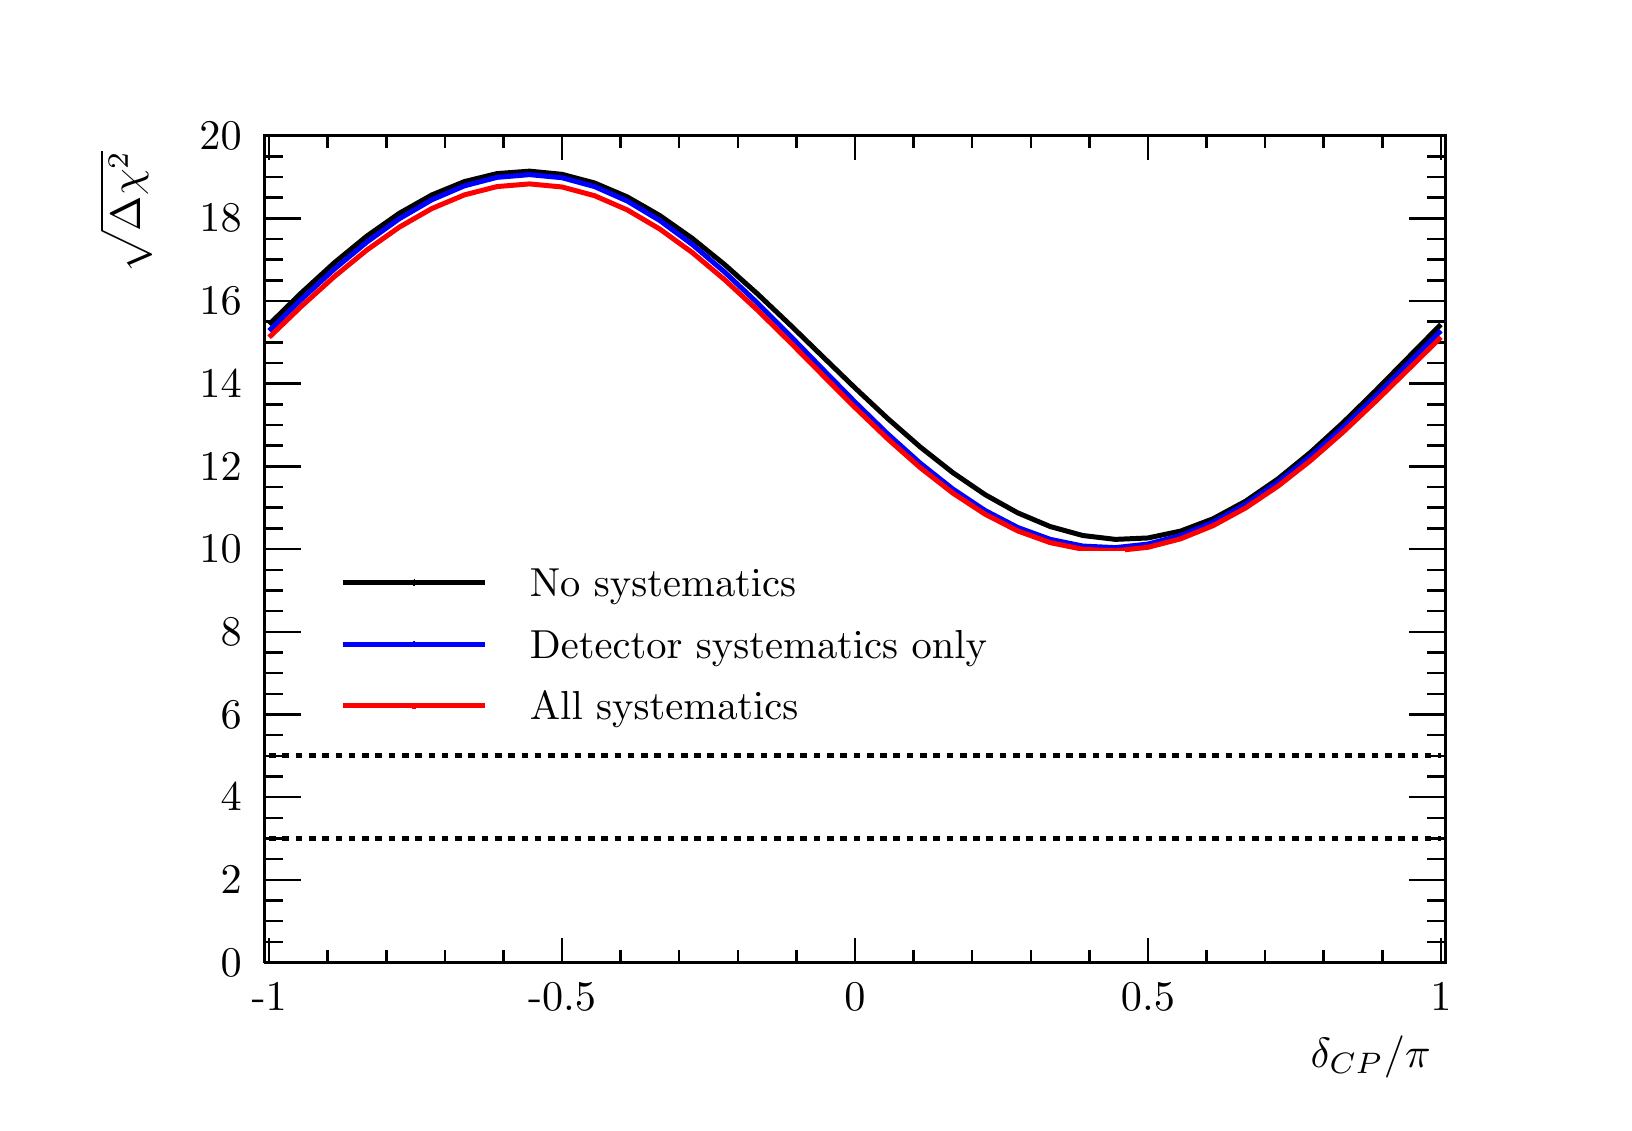
\begin{tikzpicture}
\pgfdeclareplotmark{cross} {
\pgfpathmoveto{\pgfpoint{-0.3\pgfplotmarksize}{\pgfplotmarksize}}
\pgfpathlineto{\pgfpoint{+0.3\pgfplotmarksize}{\pgfplotmarksize}}
\pgfpathlineto{\pgfpoint{+0.3\pgfplotmarksize}{0.3\pgfplotmarksize}}
\pgfpathlineto{\pgfpoint{+1\pgfplotmarksize}{0.3\pgfplotmarksize}}
\pgfpathlineto{\pgfpoint{+1\pgfplotmarksize}{-0.3\pgfplotmarksize}}
\pgfpathlineto{\pgfpoint{+0.3\pgfplotmarksize}{-0.3\pgfplotmarksize}}
\pgfpathlineto{\pgfpoint{+0.3\pgfplotmarksize}{-1.\pgfplotmarksize}}
\pgfpathlineto{\pgfpoint{-0.3\pgfplotmarksize}{-1.\pgfplotmarksize}}
\pgfpathlineto{\pgfpoint{-0.3\pgfplotmarksize}{-0.3\pgfplotmarksize}}
\pgfpathlineto{\pgfpoint{-1.\pgfplotmarksize}{-0.3\pgfplotmarksize}}
\pgfpathlineto{\pgfpoint{-1.\pgfplotmarksize}{0.3\pgfplotmarksize}}
\pgfpathlineto{\pgfpoint{-0.3\pgfplotmarksize}{0.3\pgfplotmarksize}}
\pgfpathclose
\pgfusepathqstroke
}
\pgfdeclareplotmark{cross*} {
\pgfpathmoveto{\pgfpoint{-0.3\pgfplotmarksize}{\pgfplotmarksize}}
\pgfpathlineto{\pgfpoint{+0.3\pgfplotmarksize}{\pgfplotmarksize}}
\pgfpathlineto{\pgfpoint{+0.3\pgfplotmarksize}{0.3\pgfplotmarksize}}
\pgfpathlineto{\pgfpoint{+1\pgfplotmarksize}{0.3\pgfplotmarksize}}
\pgfpathlineto{\pgfpoint{+1\pgfplotmarksize}{-0.3\pgfplotmarksize}}
\pgfpathlineto{\pgfpoint{+0.3\pgfplotmarksize}{-0.3\pgfplotmarksize}}
\pgfpathlineto{\pgfpoint{+0.3\pgfplotmarksize}{-1.\pgfplotmarksize}}
\pgfpathlineto{\pgfpoint{-0.3\pgfplotmarksize}{-1.\pgfplotmarksize}}
\pgfpathlineto{\pgfpoint{-0.3\pgfplotmarksize}{-0.3\pgfplotmarksize}}
\pgfpathlineto{\pgfpoint{-1.\pgfplotmarksize}{-0.3\pgfplotmarksize}}
\pgfpathlineto{\pgfpoint{-1.\pgfplotmarksize}{0.3\pgfplotmarksize}}
\pgfpathlineto{\pgfpoint{-0.3\pgfplotmarksize}{0.3\pgfplotmarksize}}
\pgfpathclose
\pgfusepathqfillstroke
}
\pgfdeclareplotmark{newstar} {
\pgfpathmoveto{\pgfqpoint{0pt}{\pgfplotmarksize}}
\pgfpathlineto{\pgfqpointpolar{44}{0.5\pgfplotmarksize}}
\pgfpathlineto{\pgfqpointpolar{18}{\pgfplotmarksize}}
\pgfpathlineto{\pgfqpointpolar{-20}{0.5\pgfplotmarksize}}
\pgfpathlineto{\pgfqpointpolar{-54}{\pgfplotmarksize}}
\pgfpathlineto{\pgfqpointpolar{-90}{0.5\pgfplotmarksize}}
\pgfpathlineto{\pgfqpointpolar{234}{\pgfplotmarksize}}
\pgfpathlineto{\pgfqpointpolar{198}{0.5\pgfplotmarksize}}
\pgfpathlineto{\pgfqpointpolar{162}{\pgfplotmarksize}}
\pgfpathlineto{\pgfqpointpolar{134}{0.5\pgfplotmarksize}}
\pgfpathclose
\pgfusepathqstroke
}
\pgfdeclareplotmark{newstar*} {
\pgfpathmoveto{\pgfqpoint{0pt}{\pgfplotmarksize}}
\pgfpathlineto{\pgfqpointpolar{44}{0.5\pgfplotmarksize}}
\pgfpathlineto{\pgfqpointpolar{18}{\pgfplotmarksize}}
\pgfpathlineto{\pgfqpointpolar{-20}{0.5\pgfplotmarksize}}
\pgfpathlineto{\pgfqpointpolar{-54}{\pgfplotmarksize}}
\pgfpathlineto{\pgfqpointpolar{-90}{0.5\pgfplotmarksize}}
\pgfpathlineto{\pgfqpointpolar{234}{\pgfplotmarksize}}
\pgfpathlineto{\pgfqpointpolar{198}{0.5\pgfplotmarksize}}
\pgfpathlineto{\pgfqpointpolar{162}{\pgfplotmarksize}}
\pgfpathlineto{\pgfqpointpolar{134}{0.5\pgfplotmarksize}}
\pgfpathclose
\pgfusepathqfillstroke
}
\definecolor{c}{rgb}{1,1,1};
\draw [color=c, fill=c] (0,0) rectangle (20,13.639);
\draw [color=c, fill=c] (3,1.77307) rectangle (18,12.2751);
\definecolor{c}{rgb}{0,0,0};
\draw [c,line width=0.9] (3,1.77307) -- (3,12.2751) -- (18,12.2751) -- (18,1.77307) -- (3,1.77307);
\definecolor{c}{rgb}{1,1,1};
\draw [color=c, fill=c] (3,1.77307) rectangle (18,12.2751);
\definecolor{c}{rgb}{0,0,0};
\draw [c,line width=0.9] (3,1.77307) -- (3,12.2751) -- (18,12.2751) -- (18,1.77307) -- (3,1.77307);
\draw [c,line width=0.9] (3,1.77307) -- (18,1.77307);
\draw [c,line width=0.9] (3.05952,2.07994) -- (3.05952,1.77307);
\draw [c,line width=0.9] (3.80357,1.9265) -- (3.80357,1.77307);
\draw [c,line width=0.9] (4.54762,1.9265) -- (4.54762,1.77307);
\draw [c,line width=0.9] (5.29167,1.9265) -- (5.29167,1.77307);
\draw [c,line width=0.9] (6.03571,1.9265) -- (6.03571,1.77307);
\draw [c,line width=0.9] (6.77976,2.07994) -- (6.77976,1.77307);
\draw [c,line width=0.9] (7.52381,1.9265) -- (7.52381,1.77307);
\draw [c,line width=0.9] (8.26786,1.9265) -- (8.26786,1.77307);
\draw [c,line width=0.9] (9.0119,1.9265) -- (9.0119,1.77307);
\draw [c,line width=0.9] (9.75595,1.9265) -- (9.75595,1.77307);
\draw [c,line width=0.9] (10.5,2.07994) -- (10.5,1.77307);
\draw [c,line width=0.9] (11.244,1.9265) -- (11.244,1.77307);
\draw [c,line width=0.9] (11.9881,1.9265) -- (11.9881,1.77307);
\draw [c,line width=0.9] (12.7321,1.9265) -- (12.7321,1.77307);
\draw [c,line width=0.9] (13.4762,1.9265) -- (13.4762,1.77307);
\draw [c,line width=0.9] (14.2202,2.07994) -- (14.2202,1.77307);
\draw [c,line width=0.9] (14.9643,1.9265) -- (14.9643,1.77307);
\draw [c,line width=0.9] (15.7083,1.9265) -- (15.7083,1.77307);
\draw [c,line width=0.9] (16.4524,1.9265) -- (16.4524,1.77307);
\draw [c,line width=0.9] (17.1964,1.9265) -- (17.1964,1.77307);
\draw [c,line width=0.9] (17.9405,2.07994) -- (17.9405,1.77307);
\draw [c,line width=0.9] (3.05952,2.07994) -- (3.05952,1.77307);
\draw [c,line width=0.9] (17.9405,2.07994) -- (17.9405,1.77307);
\draw [anchor=base] (3.05952,1.15931) node[scale=1.52731, color=c, rotate=0]{-1};
\draw [anchor=base] (6.77976,1.15931) node[scale=1.52731, color=c, rotate=0]{-0.5};
\draw [anchor=base] (10.5,1.15931) node[scale=1.52731, color=c, rotate=0]{0};
\draw [anchor=base] (14.2202,1.15931) node[scale=1.52731, color=c, rotate=0]{0.5};
\draw [anchor=base] (17.9405,1.15931) node[scale=1.52731, color=c, rotate=0]{1};
\draw [anchor= east] (18,0.572837) node[scale=1.52731, color=c, rotate=0]{$\delta_{CP} / \pi$};
\draw [c,line width=0.9] (3,12.2751) -- (18,12.2751);
\draw [c,line width=0.9] (3.05952,11.9682) -- (3.05952,12.2751);
\draw [c,line width=0.9] (3.80357,12.1216) -- (3.80357,12.2751);
\draw [c,line width=0.9] (4.54762,12.1216) -- (4.54762,12.2751);
\draw [c,line width=0.9] (5.29167,12.1216) -- (5.29167,12.2751);
\draw [c,line width=0.9] (6.03571,12.1216) -- (6.03571,12.2751);
\draw [c,line width=0.9] (6.77976,11.9682) -- (6.77976,12.2751);
\draw [c,line width=0.9] (7.52381,12.1216) -- (7.52381,12.2751);
\draw [c,line width=0.9] (8.26786,12.1216) -- (8.26786,12.2751);
\draw [c,line width=0.9] (9.0119,12.1216) -- (9.0119,12.2751);
\draw [c,line width=0.9] (9.75595,12.1216) -- (9.75595,12.2751);
\draw [c,line width=0.9] (10.5,11.9682) -- (10.5,12.2751);
\draw [c,line width=0.9] (11.244,12.1216) -- (11.244,12.2751);
\draw [c,line width=0.9] (11.9881,12.1216) -- (11.9881,12.2751);
\draw [c,line width=0.9] (12.7321,12.1216) -- (12.7321,12.2751);
\draw [c,line width=0.9] (13.4762,12.1216) -- (13.4762,12.2751);
\draw [c,line width=0.9] (14.2202,11.9682) -- (14.2202,12.2751);
\draw [c,line width=0.9] (14.9643,12.1216) -- (14.9643,12.2751);
\draw [c,line width=0.9] (15.7083,12.1216) -- (15.7083,12.2751);
\draw [c,line width=0.9] (16.4524,12.1216) -- (16.4524,12.2751);
\draw [c,line width=0.9] (17.1964,12.1216) -- (17.1964,12.2751);
\draw [c,line width=0.9] (17.9405,11.9682) -- (17.9405,12.2751);
\draw [c,line width=0.9] (3.05952,11.9682) -- (3.05952,12.2751);
\draw [c,line width=0.9] (17.9405,11.9682) -- (17.9405,12.2751);
\draw [c,line width=0.9] (3,1.77307) -- (3,12.2751);
\draw [c,line width=0.9] (3.462,1.77307) -- (3,1.77307);
\draw [c,line width=0.9] (3.231,2.03562) -- (3,2.03562);
\draw [c,line width=0.9] (3.231,2.29817) -- (3,2.29817);
\draw [c,line width=0.9] (3.231,2.56072) -- (3,2.56072);
\draw [c,line width=0.9] (3.462,2.82327) -- (3,2.82327);
\draw [c,line width=0.9] (3.231,3.08582) -- (3,3.08582);
\draw [c,line width=0.9] (3.231,3.34837) -- (3,3.34837);
\draw [c,line width=0.9] (3.231,3.61092) -- (3,3.61092);
\draw [c,line width=0.9] (3.462,3.87347) -- (3,3.87347);
\draw [c,line width=0.9] (3.231,4.13602) -- (3,4.13602);
\draw [c,line width=0.9] (3.231,4.39857) -- (3,4.39857);
\draw [c,line width=0.9] (3.231,4.66112) -- (3,4.66112);
\draw [c,line width=0.9] (3.462,4.92367) -- (3,4.92367);
\draw [c,line width=0.9] (3.231,5.18622) -- (3,5.18622);
\draw [c,line width=0.9] (3.231,5.44877) -- (3,5.44877);
\draw [c,line width=0.9] (3.231,5.71132) -- (3,5.71132);
\draw [c,line width=0.9] (3.462,5.97387) -- (3,5.97387);
\draw [c,line width=0.9] (3.231,6.23642) -- (3,6.23642);
\draw [c,line width=0.9] (3.231,6.49897) -- (3,6.49897);
\draw [c,line width=0.9] (3.231,6.76152) -- (3,6.76152);
\draw [c,line width=0.9] (3.462,7.02407) -- (3,7.02407);
\draw [c,line width=0.9] (3.231,7.28662) -- (3,7.28662);
\draw [c,line width=0.9] (3.231,7.54917) -- (3,7.54917);
\draw [c,line width=0.9] (3.231,7.81172) -- (3,7.81172);
\draw [c,line width=0.9] (3.462,8.07427) -- (3,8.07427);
\draw [c,line width=0.9] (3.231,8.33682) -- (3,8.33682);
\draw [c,line width=0.9] (3.231,8.59937) -- (3,8.59937);
\draw [c,line width=0.9] (3.231,8.86192) -- (3,8.86192);
\draw [c,line width=0.9] (3.462,9.12447) -- (3,9.12447);
\draw [c,line width=0.9] (3.231,9.38702) -- (3,9.38702);
\draw [c,line width=0.9] (3.231,9.64957) -- (3,9.64957);
\draw [c,line width=0.9] (3.231,9.91212) -- (3,9.91212);
\draw [c,line width=0.9] (3.462,10.1747) -- (3,10.1747);
\draw [c,line width=0.9] (3.231,10.4372) -- (3,10.4372);
\draw [c,line width=0.9] (3.231,10.6998) -- (3,10.6998);
\draw [c,line width=0.9] (3.231,10.9623) -- (3,10.9623);
\draw [c,line width=0.9] (3.462,11.2249) -- (3,11.2249);
\draw [c,line width=0.9] (3.231,11.4874) -- (3,11.4874);
\draw [c,line width=0.9] (3.231,11.75) -- (3,11.75);
\draw [c,line width=0.9] (3.231,12.0125) -- (3,12.0125);
\draw [c,line width=0.9] (3.462,12.2751) -- (3,12.2751);
\draw [anchor= east] (2.9,1.77307) node[scale=1.52731, color=c, rotate=0]{0};
\draw [anchor= east] (2.9,2.82327) node[scale=1.52731, color=c, rotate=0]{2};
\draw [anchor= east] (2.9,3.87347) node[scale=1.52731, color=c, rotate=0]{4};
\draw [anchor= east] (2.9,4.92367) node[scale=1.52731, color=c, rotate=0]{6};
\draw [anchor= east] (2.9,5.97387) node[scale=1.52731, color=c, rotate=0]{8};
\draw [anchor= east] (2.9,7.02407) node[scale=1.52731, color=c, rotate=0]{10};
\draw [anchor= east] (2.9,8.07427) node[scale=1.52731, color=c, rotate=0]{12};
\draw [anchor= east] (2.9,9.12447) node[scale=1.52731, color=c, rotate=0]{14};
\draw [anchor= east] (2.9,10.1747) node[scale=1.52731, color=c, rotate=0]{16};
\draw [anchor= east] (2.9,11.2249) node[scale=1.52731, color=c, rotate=0]{18};
\draw [anchor= east] (2.9,12.2751) node[scale=1.52731, color=c, rotate=0]{20};
\draw [anchor= east] (1.24,12.2751) node[scale=1.52731, color=c, rotate=90]{$\sqrt{ \Delta \chi^{2} }$};
\draw [c,line width=0.9] (18,1.77307) -- (18,12.2751);
\draw [c,line width=0.9] (17.538,1.77307) -- (18,1.77307);
\draw [c,line width=0.9] (17.769,2.03562) -- (18,2.03562);
\draw [c,line width=0.9] (17.769,2.29817) -- (18,2.29817);
\draw [c,line width=0.9] (17.769,2.56072) -- (18,2.56072);
\draw [c,line width=0.9] (17.538,2.82327) -- (18,2.82327);
\draw [c,line width=0.9] (17.769,3.08582) -- (18,3.08582);
\draw [c,line width=0.9] (17.769,3.34837) -- (18,3.34837);
\draw [c,line width=0.9] (17.769,3.61092) -- (18,3.61092);
\draw [c,line width=0.9] (17.538,3.87347) -- (18,3.87347);
\draw [c,line width=0.9] (17.769,4.13602) -- (18,4.13602);
\draw [c,line width=0.9] (17.769,4.39857) -- (18,4.39857);
\draw [c,line width=0.9] (17.769,4.66112) -- (18,4.66112);
\draw [c,line width=0.9] (17.538,4.92367) -- (18,4.92367);
\draw [c,line width=0.9] (17.769,5.18622) -- (18,5.18622);
\draw [c,line width=0.9] (17.769,5.44877) -- (18,5.44877);
\draw [c,line width=0.9] (17.769,5.71132) -- (18,5.71132);
\draw [c,line width=0.9] (17.538,5.97387) -- (18,5.97387);
\draw [c,line width=0.9] (17.769,6.23642) -- (18,6.23642);
\draw [c,line width=0.9] (17.769,6.49897) -- (18,6.49897);
\draw [c,line width=0.9] (17.769,6.76152) -- (18,6.76152);
\draw [c,line width=0.9] (17.538,7.02407) -- (18,7.02407);
\draw [c,line width=0.9] (17.769,7.28662) -- (18,7.28662);
\draw [c,line width=0.9] (17.769,7.54917) -- (18,7.54917);
\draw [c,line width=0.9] (17.769,7.81172) -- (18,7.81172);
\draw [c,line width=0.9] (17.538,8.07427) -- (18,8.07427);
\draw [c,line width=0.9] (17.769,8.33682) -- (18,8.33682);
\draw [c,line width=0.9] (17.769,8.59937) -- (18,8.59937);
\draw [c,line width=0.9] (17.769,8.86192) -- (18,8.86192);
\draw [c,line width=0.9] (17.538,9.12447) -- (18,9.12447);
\draw [c,line width=0.9] (17.769,9.38702) -- (18,9.38702);
\draw [c,line width=0.9] (17.769,9.64957) -- (18,9.64957);
\draw [c,line width=0.9] (17.769,9.91212) -- (18,9.91212);
\draw [c,line width=0.9] (17.538,10.1747) -- (18,10.1747);
\draw [c,line width=0.9] (17.769,10.4372) -- (18,10.4372);
\draw [c,line width=0.9] (17.769,10.6998) -- (18,10.6998);
\draw [c,line width=0.9] (17.769,10.9623) -- (18,10.9623);
\draw [c,line width=0.9] (17.538,11.2249) -- (18,11.2249);
\draw [c,line width=0.9] (17.769,11.4874) -- (18,11.4874);
\draw [c,line width=0.9] (17.769,11.75) -- (18,11.75);
\draw [c,line width=0.9] (17.769,12.0125) -- (18,12.0125);
\draw [c,line width=0.9] (17.538,12.2751) -- (18,12.2751);
\draw [c,line width=1.8] (3.05952,9.87672) -- (3.47288,10.2815) -- (3.88624,10.6592) -- (4.2996,10.9982) -- (4.71296,11.2885) -- (5.12632,11.5217) -- (5.53968,11.6913) -- (5.95304,11.7928) -- (6.3664,11.8237) -- (6.77976,11.7834) -- (7.19312,11.6734)
 -- (7.60648,11.4972) -- (8.01984,11.2604) -- (8.4332,10.9701) -- (8.84656,10.6353) -- (9.25992,10.2662) -- (9.67328,9.87424) -- (10.0866,9.47163) -- (10.5,9.07076) -- (10.9134,8.68383) -- (11.3267,8.32228) -- (11.7401,7.99633) -- (12.1534,7.71458)
 -- (12.5668,7.48395) -- (12.9802,7.30981) -- (13.3935,7.1964) -- (13.8069,7.14723) -- (14.2202,7.16522) -- (14.6336,7.25235) -- (15.047,7.40882) -- (15.4603,7.63219) -- (15.8737,7.91683) -- (16.287,8.25391) -- (16.7004,8.63202) -- (17.1138,9.03796)
 -- (17.5271,9.4576) -- (17.9405,9.87672);
\definecolor{c}{rgb}{0,0,1};
\draw [c,line width=1.8] (3.05952,9.79587) -- (3.47288,10.1994) -- (3.88624,10.5791) -- (4.2996,10.9228) -- (4.71296,11.2197) -- (5.12632,11.4603) -- (5.53968,11.6372) -- (5.95304,11.7447) -- (6.3664,11.7794) -- (6.77976,11.74) -- (7.19312,11.6274)
 -- (7.60648,11.4448) -- (8.01984,11.1974) -- (8.4332,10.8928) -- (8.84656,10.5401) -- (9.25992,10.1505) -- (9.67328,9.73653) -- (10.0866,9.3119) -- (10.5,8.89092) -- (10.9134,8.48792) -- (11.3267,8.11642) -- (11.7401,7.78841) -- (12.1534,7.51353) --
 (12.5668,7.29862) -- (12.9802,7.14766) -- (13.3935,7.06231) -- (13.8069,7.0426) -- (14.2202,7.08763) -- (14.6336,7.19608) -- (15.047,7.366) -- (15.4603,7.59438) -- (15.8737,7.87661) -- (16.287,8.20608) -- (16.7004,8.57408) -- (17.1138,8.97) --
 (17.5271,9.38163) -- (17.9405,9.79587);
\definecolor{c}{rgb}{1,0,0};
\draw [c,line width=1.8] (3.05952,9.71362) -- (3.47288,10.1103) -- (3.88624,10.4835) -- (4.2996,10.8212) -- (4.71296,11.1127) -- (5.12632,11.349) -- (5.53968,11.5224) -- (5.95304,11.6278) -- (6.3664,11.6616) -- (6.77976,11.6226) -- (7.19312,11.5117)
 -- (7.60648,11.3322) -- (8.01984,11.089) -- (8.4332,10.7896) -- (8.84656,10.443) -- (9.25992,10.06) -- (9.67328,9.65306) -- (10.0866,9.23554) -- (10.5,8.82152) -- (10.9134,8.42506) -- (11.3267,8.05949) -- (11.7401,7.73661) -- (12.1534,7.46593) --
 (12.5668,7.25424) -- (12.9802,7.10554) -- (13.3935,7.0215) -- (13.8069,7.00215) -- (14.2202,7.04665) -- (14.6336,7.15366) -- (15.047,7.32124) -- (15.4603,7.54639) -- (15.8737,7.82451) -- (16.287,8.14909) -- (16.7004,8.51147) -- (17.1138,8.90117) --
 (17.5271,9.30619) -- (17.9405,9.71362);
\definecolor{c}{rgb}{0,0,0};
\draw [c,dash pattern=on 2.40pt off 2.40pt ,line width=1.8] (3.05952,3.34837) -- (17.9405,3.34837);
\draw [c,dash pattern=on 2.40pt off 2.40pt ,line width=1.8] (3.05952,4.39857) -- (17.9405,4.39857);
\definecolor{c}{rgb}{1,1,1};
\draw [color=c, fill=c] (3.61032,4.64183) rectangle (13.9255,6.9914);
\definecolor{c}{rgb}{0,0,0};
\draw [anchor=base west] (6.18911,6.42359) node[scale=1.46368, color=c, rotate=0]{No systematics};
\definecolor{c}{rgb}{1,1,1};
\draw [c, fill=c] (3.99713,6.32569) -- (5.80229,6.32569) -- (5.80229,6.87393) -- (3.99713,6.87393);
\definecolor{c}{rgb}{0,0,0};
\draw [c,line width=1.8] (3.99713,6.59981) -- (5.80229,6.59981);
\foreach \P in {(4.89971,6.59981)}{\draw[mark options={color=c,fill=c},mark size=2.402402pt, line width=0.000000pt, mark=*,mark size=1pt] plot coordinates {\P};}
\draw [anchor=base west] (6.18911,5.6404) node[scale=1.46368, color=c, rotate=0]{Detector systematics only};
\definecolor{c}{rgb}{1,1,1};
\draw [c, fill=c] (3.99713,5.5425) -- (5.80229,5.5425) -- (5.80229,6.09074) -- (3.99713,6.09074);
\definecolor{c}{rgb}{0,0,1};
\draw [c,line width=1.8] (3.99713,5.81662) -- (5.80229,5.81662);
\foreach \P in {(4.89971,5.81662)}{\draw[mark options={color=c,fill=c},mark size=2.402402pt, line width=0.000000pt, mark=*,mark size=1pt] plot coordinates {\P};}
\definecolor{c}{rgb}{0,0,0};
\draw [anchor=base west] (6.18911,4.85721) node[scale=1.46368, color=c, rotate=0]{All systematics};
\definecolor{c}{rgb}{1,1,1};
\draw [c, fill=c] (3.99713,4.75931) -- (5.80229,4.75931) -- (5.80229,5.30755) -- (3.99713,5.30755);
\definecolor{c}{rgb}{1,0,0};
\draw [c,line width=1.8] (3.99713,5.03343) -- (5.80229,5.03343);
\foreach \P in {(4.89971,5.03343)}{\draw[mark options={color=c,fill=c},mark size=2.402402pt, line width=0.000000pt, mark=*,mark size=1pt] plot coordinates {\P};}
\end{tikzpicture}
